\documentclass[a4paper,12pt]{article}
\usepackage{array}
\usepackage[utf8]{inputenc}
\usepackage[spanish]{babel}
\usepackage{graphicx}
\usepackage{tabulary}
\usepackage{tabularx}
\usepackage{slashbox}
\usepackage{rotating}

% control de márgenes
\usepackage{anysize} 
% Controla los márgenes {izquierda}{derecha}{arriba}{abajo}.
\marginsize{3cm}{2cm}{2cm}{2cm}



% cabecera y pie
\usepackage{fancyhdr} % activamos el paquete
\pagestyle{fancy} % seleccionamos un estilo
\lhead{Seminario de Sistemas Embebidos - FiUBA} % texto izquierda de la cabecera
\chead{} % texto centro de la cabecera
\rhead{TP freeRTOS} 
\lfoot{Bos - Petrella} % texto izquierda del pie
\cfoot{} 
\rfoot{pág. \thepage} % texto derecha del pie
\renewcommand{\headrulewidth}{0.4pt} % grosor de la línea de la cabecera
\renewcommand{\footrulewidth}{0.4pt} % grosor de la línea del pie


\begin{document}

\thispagestyle{empty}

\begin{center}
	
\includegraphics[width=0.2\textwidth,angle=0]{./imagenes/logo-facu.png}\\
	\huge{{Universidad de Buenos Aires}}\\
	\huge{{Facultad de Ingeniería}}\\
	\vspace{2.2cm}
	\Huge{\textbf{Seminario de Sistemas Embebidos}}\\
	\vspace{0.5cm}
	\Large{\textbf{TP freeRTOS}}\\
	\vspace{1.5cm}
	\Large{$2^{do}$ cuatrimestre de 2012}\\
	\vspace{2cm}	
\end{center}

\vfill
\begin{flushright}
		\textbf{Alumnos:}  Matías Petrella (68405)\\
		 Patricio Bos (81163)\\
		\textbf{Fecha:}  22/02/13\\
\end{flushright}
\newpage



\tableofcontents
\thispagestyle{empty}
\newpage

%------------------------------------------------------------------------------------------------
%------------------------------------------------------------------------------------------------
\section{Objetivo}
%------------------------------------------------------------------------------------------------
%------------------------------------------------------------------------------------------------

El LPCXpresso es un toolchain completo de desarrollo y evaluación para microcontroladores de NXP.
Se compone de los siguientes elementos:
\begin{itemize}
\item LPCXpresso IDE y herramientas de desarrollo
\item LPCXpresso target board (stick)
\item LPCXpresso Baseboard EA-XPR-021
\end{itemize}

Se propone utilizar el entorno de desarrollo LPCXpresso para implementar las siguientes tareas sobre el sistema operativo en tiempo real \textbf{freeRTOS}.

\begin{itemize}
\item \textbf{Tarea 1:}\\
De forma periódica cada 100ms se debe enviar por la UART3 el mensaje constante "Tarea 1 - Enviando información por la UART 3”.
\item \textbf{Tarea 2:}\\
Realizar un eco de los caracteres recibidos por la UART3 utilizando un semáforo para sincronizar la tarea  con la interrupción del puerto serie.
\item \textbf{Tarea 3:}\\
Se debe inicializar el RTC en 00:00:00 y habilitar una interrupción externa por pulsador del BaseBoard. Cuando el pulsador se oprime se debe utilizar una cola para pasar el dato del RTC a una función que lo envie por la UART3
\end{itemize}

Para enviar información por la UART se debe implementar una función Enviar UART con el siguiente encabezado:

\begin{center}
void UART3\_Enviar (uint8\_t* buffer, uint32\_t size);
\end{center}

%------------------------------------------------------------------------------------------------
%------------------------------------------------------------------------------------------------
\newpage
\section{Desarrollo}
%------------------------------------------------------------------------------------------------
%------------------------------------------------------------------------------------------------
\subsection{Introduccion} 
Para cumplir los objetivos planteados se hará uso de los siguientes conceptos:\\
\begin{itemize}

\item {\textbf{cola:}}
Las colas son los elementos con los que se establecen todas las comunicaciones dentro del entorno freeRTOS.  Pueden contener un número finito de elementos de un tamaño fijo.  Cuando se crean se definen dos parámetros: la cantidad de elementos y el tamaño de los mismos.  Normalmente se utilizan como un buffer FIFO, aunque se puede leer en ambos sentidos.

\item {\textbf{semáforo:}}
Un semáforo binario puede ser considerado como una cola de 1 solo elemento cuando se lo usa para sincronizar un evento con una tarea de procesamiento de la misma.

\item {\textbf{mutex:}}

Es un tipo particular de semáforo binario que se utiliza para bloquear el acceso a un recurso compartido por  mas una tarea.  Cuando se utiliza un mutex se puede evitar que una tarea de mayor prioridad deje en un estado inconsistente el uso de un recurso por parte de una tarea de menor prioridad.  Por ejemplo un mensaje que se este imprimiendo en un display.  La desventaja es que ocurre una inversión de prioridades ya que una tarea de menor prioridad le impede el acceso al procesador a una de mayor prioridad. Los mutex se distinguen de los semáforos en que cada vez que una función lo toma, debe darlo al finalizar de la utilización del recurso.\\

En el presente trabajo se utilizará un mutex cada vez que se quiera enviar información por la UART.\\

\end{itemize}

\subsection{Includes, prototípos y variables globales}

\begin{verbatim}
/* FreeRTOS.org includes. */
#include "FreeRTOS.h"
#include "task.h"
#include "semphr.h"
#include "queue.h"

/* Demo includes. */
#include "basic_io.h"

#ifdef __USE_CMSIS
#include "LPC17xx.h"
#include "lpc17xx_uart.h"
#include "lpc17xx_pinsel.h"
#include "lpc17xx_rtc.h"
#include "lpc_types.h"
#endif

#include <string.h>
#include <cr_section_macros.h>
#include <NXP/crp.h>
#include <math.h>

/* The tasks to be created. */
static void vPeriodicTask1(void);
static void vAsincronicTask2(void);
static void vAsincronicTask3(void);

void vSetupRtc(void);
void vSetupIntExt(void);
void vSetupUart3(void);
void UART3_Enviar(unsigned char* buffer, uint32_t size);

/* Declare a variable of type xSemaphoreHandle. This is 
 * used to reference the semaphore that is used to synchronize
 * a task with an interrupt. */
xSemaphoreHandle xCountingSemaphore;

/* Declare a variable of type xSemaphoreHandle. This is 
 * used to reference the mutex type semaphore that is used
 * to ensure mutual exclusive access to UART3. */
xSemaphoreHandle xMutex;

/* Declare a variable of type xQueueHandle. This is used to
 * store the queue
 * that is accessed by task 3. */
xQueueHandle xQueue;

const char welcome[]={"LPC1769 encendido...UART3 configurada\r\n"};
const char TextForPeriodicTask1[]={"Tarea 1 - 
							Enviando informacion por la UART3\n\r"};
const char TextForTask2[]={"Tarea 2 - Caracter recibido: "};
const char TextForTask3[]={"Tarea 3 - "};
unsigned char datoString[]={"xx:xx:xx"};

unsigned char RxBuffer;

static RTC_TIME_Type localTime;
\end{verbatim}

\subsection{Funciones de configuración}

Se crean funciones específicas de configuración de los periféricos que se ejecutan por única vez antes de la llamada al \textit{schedule}.  Estas son:

\begin{itemize}

\item {\textbf{void vSetupRtc(void)}}

{\begin{verbatim}
void vSetupRtc()
{
	/* RTC init module*/
	RTC_Init(LPC_RTC);

	/* Enable rtc (starts the tick counter) */
	RTC_ResetClockTickCounter(LPC_RTC);
	RTC_Cmd(LPC_RTC, ENABLE);

	/* Set current time for RTC
	 * Current time is 00:00:00 AM, 2013-01-01
	 */
	RTC_SetTime(LPC_RTC, RTC_TIMETYPE_SECOND, 0);
	RTC_SetTime(LPC_RTC, RTC_TIMETYPE_MINUTE, 0);
	RTC_SetTime(LPC_RTC, RTC_TIMETYPE_HOUR, 0);
	RTC_SetTime(LPC_RTC, RTC_TIMETYPE_MONTH, 1);
	RTC_SetTime(LPC_RTC, RTC_TIMETYPE_YEAR, 2013);
	RTC_SetTime(LPC_RTC, RTC_TIMETYPE_DAYOFMONTH, 1);
	/* Get and print current time */
	RTC_GetFullTime(LPC_RTC, &localTime);
}
\end{verbatim}}

\item {\textbf{void vSetupIntExt(void)}}

\begin{verbatim}
void vSetupIntExt()
{
	// Configure EINT0 to detect
	// set P2.10 as EINT0
	LPC_PINCON->PINSEL4 = 0x00100000;
	// Port 2.10 is rising edge .
	LPC_GPIOINT->IO2IntEnR = 0x400;
	// INT0 edge trigger
	LPC_SC->EXTMODE = 0x00000001;
	// INT0 is rising edge
	LPC_SC->EXTPOLAR = 0x00000001;
	NVIC_EnableIRQ(EINT0_IRQn);
}
\end{verbatim}

\item {\textbf{void vSetupUart3(void)}}

\begin{verbatim}
void vSetupUart3()
{
	PINSEL_CFG_Type PinCfg;

	PinCfg.Funcnum = PINSEL_FUNC_2;
	PinCfg.OpenDrain = PINSEL_PINMODE_NORMAL;
	PinCfg.Pinmode = PINSEL_PINMODE_PULLUP;
	PinCfg.Pinnum = PINSEL_PIN_0;
	PinCfg.Portnum = PINSEL_PORT_0;

	PINSEL_ConfigPin(&PinCfg);
	PinCfg.Pinnum = PINSEL_PIN_1;
	PINSEL_ConfigPin(&PinCfg);

	UART_CFG_Type UARTConfigStruct;
	UARTConfigStruct.Baud_rate = 115200;
	UARTConfigStruct.Databits = UART_DATABIT_8;
	UARTConfigStruct.Parity = UART_PARITY_NONE;
	UARTConfigStruct.Stopbits = UART_STOPBIT_1;
	UART_Init(LPC_UART3, &UARTConfigStruct);
	UART_TxCmd(LPC_UART3, ENABLE);

	UART_IntConfig(LPC_UART3, UART_INTCFG_RBR, ENABLE);
	NVIC_EnableIRQ(UART3_IRQn);

	/* mensaje de startup. No tomo el semáforo xMutex
	 * porque todavía no arrancó el schedule */
	UART3_Enviar(welcome,strlen(welcome));
}
\end{verbatim}

\end{itemize}

\subsection{Enviar\_UART3}
Para enviar información por la UART3 se establece una función que toma un puntero a char donde se encuentra la información a transmitir por la UART como primer parámetro y la cantidad de elementos como segundo.
\begin{verbatim}
void UART3_Enviar(unsigned char* buffer, uint32_t size)
{
	UART_Send(LPC_UART3, buffer, size, BLOCKING);

}
\end{verbatim} 

\subsection{Tareas}

\begin{itemize}

\item {\textbf{Tarea 1:}}

Se crea la tarea 1 con los siguientes parámetros:

\begin{center}
\textit{xTaskCreate( vPeriodicTask1, "Tarea1", 240, NULL, 1, NULL );}
\end{center}

Se inicializa una variable de tipo \textit{portTickType} llamada \textit{xLastWakeTime} con el valor actual de ticks al momento de ejecución de la tarea 1.  Esta variable sirve como parámetro para la función vTaskDelayUntil() para especificar la cantidad exacta de ticks que la tarea debe esperar en el estado \textit{bloqueado} antes de pasar al estado \textit{ready}.  De esta manera se puede asegurar una ejecución periódica de la tarea.

\begin{verbatim}
static void vPeriodicTask1( void *pvParameters )
{
	portTickType xLastWakeTime;
	
	xLastWakeTime = xTaskGetTickCount();

	/* As per most tasks, this task is implemented in an infinite loop. */
	for( ;; )
	{
		xSemaphoreTake(xMutex,portMAX_DELAY);

		/* Envia por la UART3 el mensaje constante. */
		UART3_Enviar(TextForPeriodicTask1,strlen(TextForPeriodicTask1));

		xSemaphoreGive(xMutex);
		
		/* queremos que la tarea se ejecute exactamente 
		 * cada 100 milisegundos. */
		vTaskDelayUntil( &xLastWakeTime, ( 100 / portTICK_RATE_MS ) );
	}
}
\end{verbatim} 

\item {\textbf{Tarea 2}}

Se crea la tarea 2 con los siguientes parámetros:

\begin{center}
\textit{xTaskCreate( vAsincronicTask2, "Tarea2", 240, NULL, 2, NULL );}
\end{center}

La tarea permanece bloqueada mientras el semáforo {\textit{xCountingSemaphore}} no este disponible. Cuando la ISR correspondiente a la UART3 lo habilita, la tarea envia el caracter recibido junto con un mensaje constante.

\begin{verbatim}
static void vAsincronicTask2()
{
	unsigned char * buffer;

	/* Inicializacion del puntero al buffer de recepcion */
	buffer = &RxBuffer;

	/* As per most tasks, this task is implemented 
	 * within an infinite loop. */
	for( ;; )
	{
	
	xSemaphoreTake( xCountingSemaphore, portMAX_DELAY );
	xSemaphoreTake(xMutex,portMAX_DELAY);

	/* Envia por la UART3 el mensaje constante. */
	UART3_Enviar(TextForTask2,strlen(TextForTask2));

	UART3_Enviar(buffer,1);
	UART_SendByte(LPC_UART3, '\n'); UART_SendByte(LPC_UART3, '\r');

	xSemaphoreGive(xMutex);
	}
}

\end{verbatim}

\item{\textbf{Tarea 3}}

Se crea la tarea 3 con los siguientes parámetros:

\begin{center}
\textit{xTaskCreate( vAsincronicTask3, "Tarea3", 240, NULL, 2, NULL );}
\end{center}

La tarea 3 permanece en el estado bloqueado hasta que haya información disponible en la cola {\textit{xQueue}}.  La ISR correspondiente al pulsador externo se encarga de escribir en dicha cola.

\begin{verbatim}
static void vAsincronicTask3( void *pvParameters )
{
	portBASE_TYPE xStatus;
	char dato[8];

	/* This task is also defined within an infinite loop. */
	for( ;; )
	{
		/* As this task unblocks immediately that data is
		 * written to the queue this
		 * call should always find the queue empty. */
		if( uxQueueMessagesWaiting( xQueue ) != 0 )
		{
			xStatus = xQueueReceive( xQueue, dato, 0 );
			xSemaphoreTake(xMutex,portMAX_DELAY);

			UART3_Enviar("RTC inicializado en ",strlen("RTC inicializado en "));

			UART3_Enviar(dato,8);
			UART_SendByte(LPC_UART3, '\n');
			UART_SendByte(LPC_UART3, '\r');

			xSemaphoreGive(xMutex);
		}

		xStatus = xQueueReceive( xQueue, dato, portMAX_DELAY );

		if( xStatus == pdPASS )
		{
			/* Data was successfully received from the queue, 
			 * print out the received value. */
			xSemaphoreTake(xMutex,portMAX_DELAY);

			UART3_Enviar(TextForTask3,strlen(TextForTask3));

			UART3_Enviar(dato,8);
			UART_SendByte(LPC_UART3, '\n');
			UART_SendByte(LPC_UART3, '\r');

			xSemaphoreGive(xMutex);
		}
	}
}
\end{verbatim}
\end{itemize}

\subsection{Routinas de interrupción}
\begin{itemize}

\item {\textbf{EINT0\_IRQHandler}}

\begin{verbatim}
void EINT0_IRQHandler ()
{
	portBASE_TYPE xHigherPriorityTaskWoken = pdFALSE;
	portBASE_TYPE xStatus;

	uint32_t seg_int,min_int,hor_int;
	char decena,unidad;

	/* se limpia la interrupcion */
	LPC_SC->EXTINT = 0x00000001;

	RTC_GetFullTime(LPC_RTC, &localTime);

	seg_int=localTime.SEC;
	min_int=localTime.MIN;
	hor_int=localTime.HOUR;

	decena=(char)floor(hor_int/10)+48;
	unidad=(char)fmod(hor_int,10)+48;
	datoString[0]=decena;
	datoString[1]=unidad;

	decena=(char)floor(min_int/10)+48;
	unidad=(char)fmod(min_int,10)+48;
	datoString[3]=decena;
	datoString[4]=unidad;

	decena=(char)floor(seg_int/10)+48;
	unidad=(char)fmod(seg_int,10)+48;
	datoString[6]=decena;
	datoString[7]=unidad;

	xStatus = xQueueSendToBack(xQueue, datoString,0);

	if (xStatus != pdPASS) {
		/* the send operation could not be completed. xQueue full?
		 * must be an error cause the queue could never contain
		 * more than 1 element */
		for(;;){
		}
	}
	
	portEND_SWITCHING_ISR( xHigherPriorityTaskWoken );
}
\end{verbatim}

\item {\textbf{UART3\_IRQHandler}}

\begin{verbatim}
void UART3_IRQHandler(void)
{
	int i;

	// Ugly Delay
	for (i=0;i<100000;i++);

	RxBuffer = UART_ReceiveByte(LPC_UART3);
	unsigned char dummy= UART_ReceiveByte(LPC_UART3);

	portBASE_TYPE xHigherPriorityTaskWoken = pdFALSE;

	/* 'Give' the semaphore to unlock tarea2 */
	xSemaphoreGiveFromISR( xCountingSemaphore, &xHigherPriorityTaskWoken );

	/* Si una tarea de igual o mayor prioridad pasa a estado ready, 
	 * xHigherPriorityTaskWoken se establece en pdTRUE y
	 * portEND_SWITCHING_ISR() asegura un cambio de contexto

	 * La instruccion para realizar un cambio de contexto 
	 * desde dentro de una ISR es la macro 
	 * portEND_SWITCHING_ISR(). No se debe usar taskYIELD()
	 * ya que no es ISRsafe	 */
	
	portEND_SWITCHING_ISR( xHigherPriorityTaskWoken );
}
\end{verbatim}

\end{itemize}

\section{Diagrama temporal}

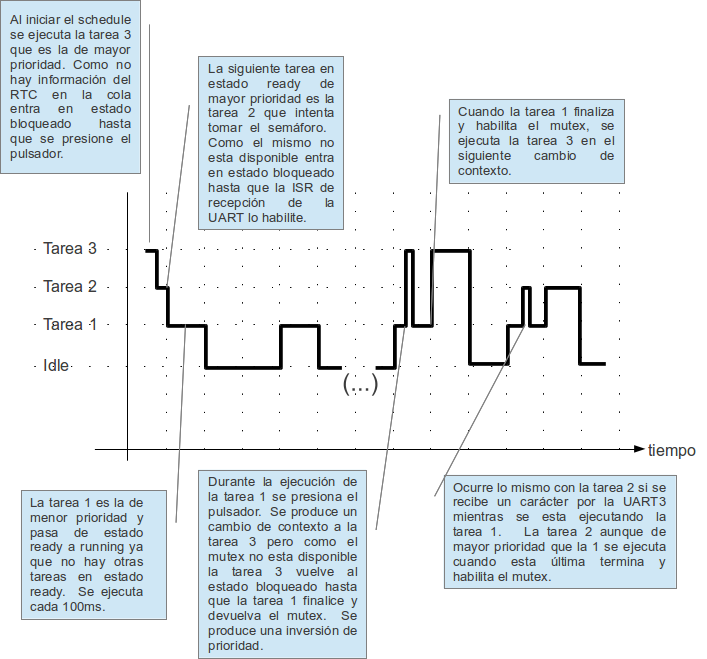
\includegraphics[width=0.9\textwidth,angle=0]{./imagenes/diagrama-temporal.png}\\

\section{Conclusiones}
Se pudo desarrollar un sistema que cumpla con todos los objetivos propuestos haciendo uso extensivo de las funciones propias del {\textit{port}} de freeRTOS para LPC1769, así como también de la librería CMSIS provista por NXP.\\
Se utilizaron funciones ISRsafe dentro de las rutinas de interrupción y se forzó el llamado al schedule al finalizar las mismas para asegurar el cambio de contexto como práctica de buena programación.
En cuanto a la elección de las prioridades, se optó por asignar prioridades distintas a cada tarea. La mas baja a la tarea periódica y la mayor a la tarea asociada al RTC.  No obstante lo cual, todas las tareas hacen uso de la UART cuya disponibilidad esta restringida a un mutex.  Por este motivo ninguna tarea es {\textit{pre-empted}} ya que tomar el mutex le asegura permanecer en estado running.


\end{document}